\documentclass{article}
\usepackage[a4paper,margin=0.7in]{geometry}
\usepackage[hidelinks]{hyperref}
\usepackage{graphicx}
\usepackage{float}
\usepackage{caption}
\usepackage{amssymb, amsmath}
\usepackage{booktabs}
\usepackage{minted}
\usepackage[most]{tcolorbox}

\setminted{
	linenos=true,
	frame=lines,
	framesep=2mm,
	fontsize=\footnotesize
}

\newcommand{\reg}[1]{\texttt{#1}}

\newtcolorbox{extra}[1][Extra]{
	breakable, colback=gray!8, colframe=gray!60,
	title={#1}, fonttitle=\bfseries\small, boxrule=0.5pt, arc=1mm
}

\newtcolorbox{pitfall}[1][Common misconception]{
	breakable, colback=red!5, colframe=red!50!black,
	title={#1}, fonttitle=\bfseries\small, boxrule=0.5pt, arc=1mm
}

\title{Operating Systems Note}
\author{}
\date{}

\begin{document}
\pagenumbering{roman}
\maketitle
\tableofcontents
\newpage
\pagenumbering{arabic}

\section{Introduction}

\subsection{Execution Model}
\begin{itemize}
	\item \textbf{Assumption:} a machine with a single-core CPU, one program counter (\reg{PC}) and one instruction register (\reg{IR}).
	\item The CPU repeatedly performs the \emph{fetch--execute} cycle: \reg{PC} holds the address of the next instruction, that instruction is fetched into \reg{IR}, and then it is executed.
	\item When an application is running, the CPU executes the application's instructions directly on the hardware, not on top of the OS. This is called running on \textbf{bare metal}.
	\item The OS is \emph{not} executing while an application runs. It only gets the CPU back through an interrupt or a system call (see Section~\ref{sec:interrupts}).
	\item So, for native (non-interpreted) code, whatever is currently running is running on bare metal.
\end{itemize}

\begin{figure}[H]
	\centering
	\begin{minipage}{0.4\textwidth}
		\centering
		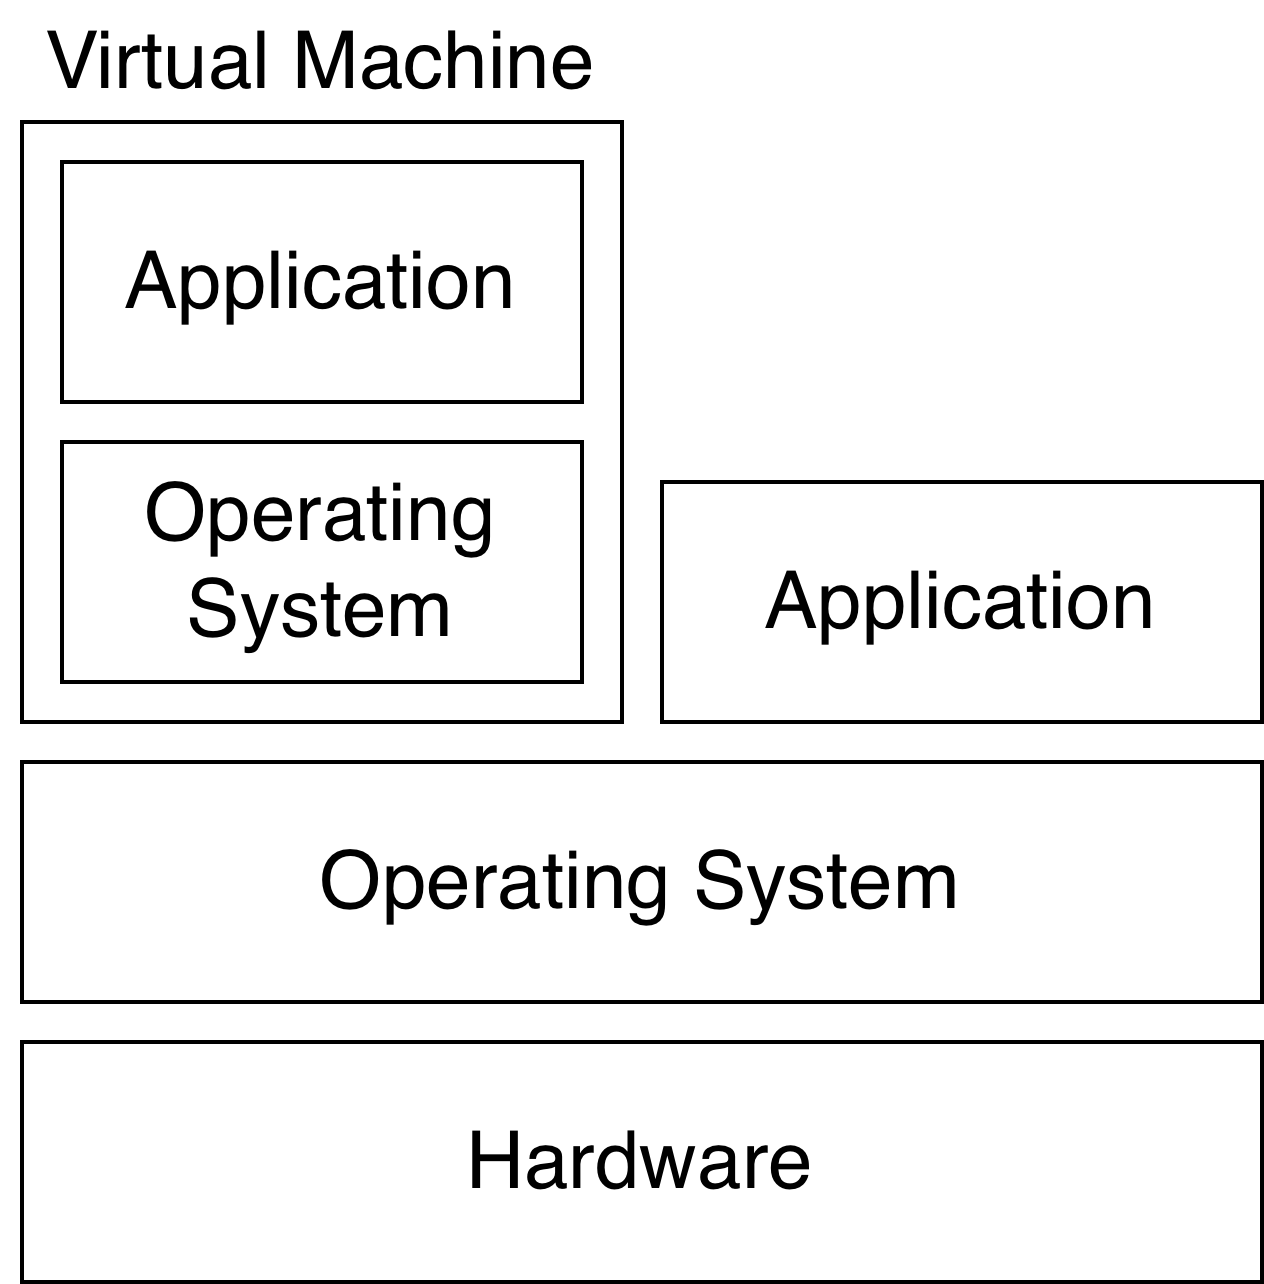
\includegraphics[width=\textwidth]{images/img-01.png}
		\caption{The usual layered depiction}
	\end{minipage}
	\hfill
	\begin{minipage}{0.4\textwidth}
		\centering
		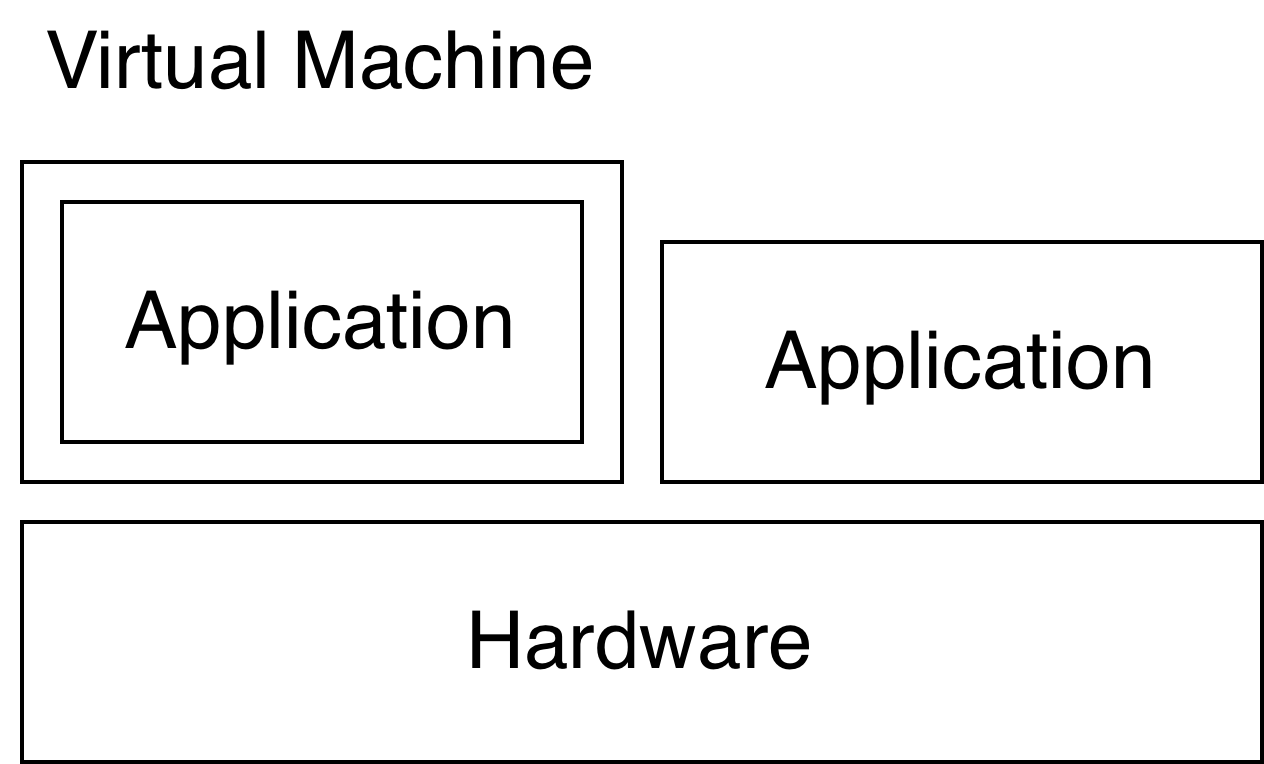
\includegraphics[width=\textwidth]{images/img-02.png}
		\caption{What is actually happening: the running code executes directly on the hardware}
	\end{minipage}
\end{figure}

\begin{extra}[Interpreters and virtual machines]
	Code run by an interpreter (e.g.\ Python, Java bytecode in a JVM) does not itself run on bare metal. The interpreter does, and it executes the code on its behalf. With hardware-assisted virtualization, a guest OS's instructions typically also run directly on the CPU, with a hypervisor stepping in only when needed.
\end{extra}

\subsection{Main Memory vs.\ Hard Disk}
\begin{itemize}
	\item Main memory is \textbf{byte addressable}.
	\item A hard disk is accessed in blocks called \textbf{sectors}. Positioning on a disk (seek and rotation) is slow compared to memory, so transferring one byte at a time would waste CPU time. Data is therefore moved in fixed-size chunks.
	\item Both are typically drawn as an array of slots for ease of understanding.
\end{itemize}

\begin{table}[H]
	\centering
	\begin{tabular}{lll}
		\toprule
		 & \textbf{Main memory (RAM)} & \textbf{Hard disk} \\
		\midrule
		Smallest access unit & 1 byte & 1 sector (commonly 512 B) \\
		Relative speed & Fast & Slow \\
		Volatile? & Yes & No \\
		\bottomrule
	\end{tabular}
\end{table}

\section{Interrupts}
\label{sec:interrupts}

\begin{figure}[H]
	\centering
	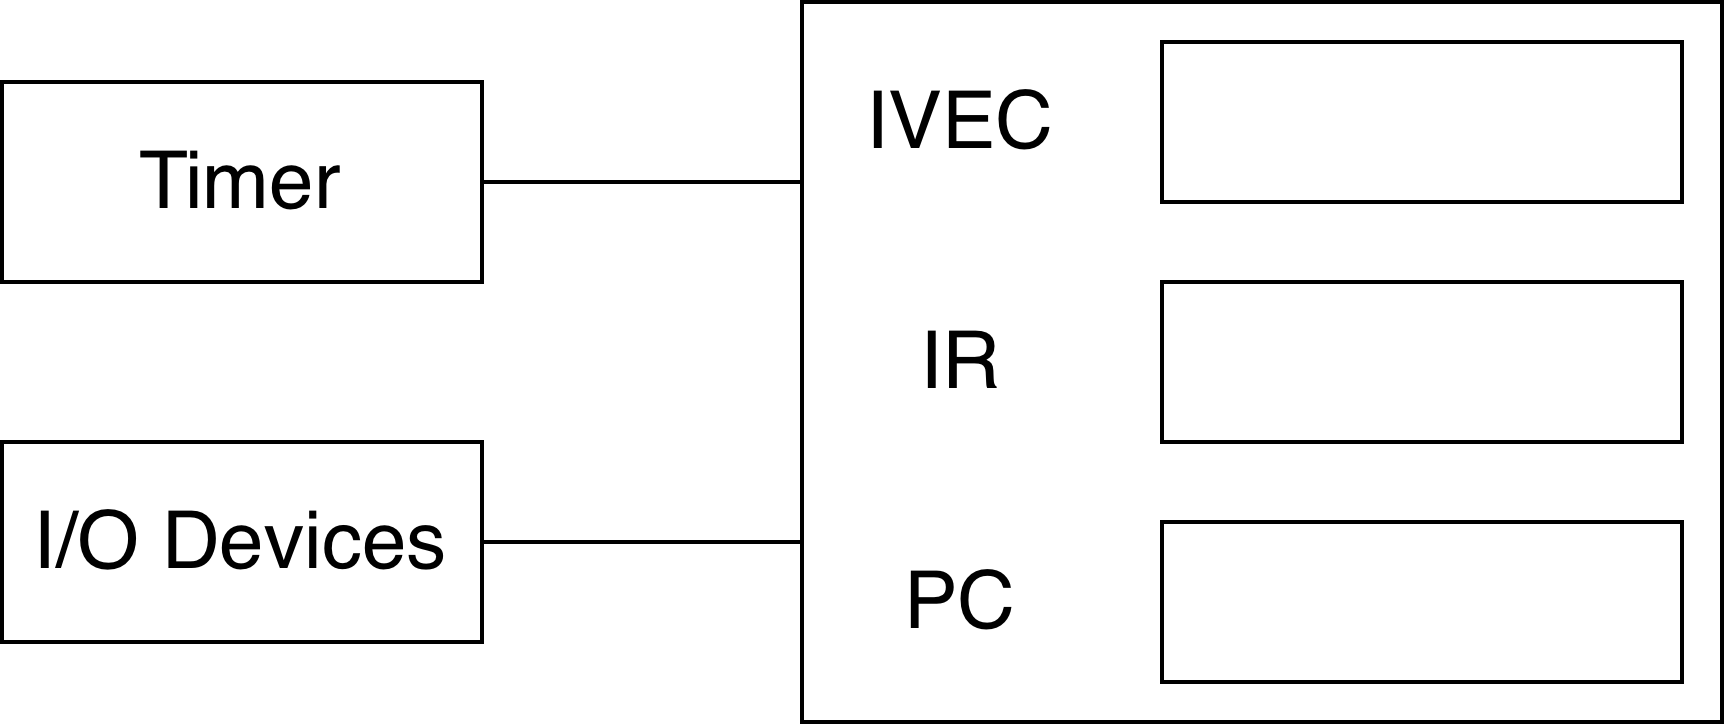
\includegraphics[width=0.4\textwidth]{images/img-03.png}
	\caption{Devices connect to the CPU through interrupt lines}
\end{figure}

\subsection{Basics}
\begin{itemize}
	\item Interrupts are signals generated by I/O devices (keyboard, mouse, \dots) or by the timer. These devices are connected to the CPU through interrupt lines.
	\item The \reg{IVEC} (interrupt vector) register holds the memory address of the first instruction of the interrupt handler. The handler is part of the OS.
\end{itemize}

\subsection{What Happens on an Interrupt}
\begin{enumerate}
	\item An application is running; the CPU is fetching its instructions.
	\item An interrupt signal arrives on an interrupt line.
	\item The value in \reg{IVEC} is copied into \reg{PC}.
	\item The next fetch therefore reads the handler's first instruction (from the OS's memory) into \reg{IR}.
	\item The handler executes, so the OS is now running.
\end{enumerate}

\begin{figure}[H]
	\centering
	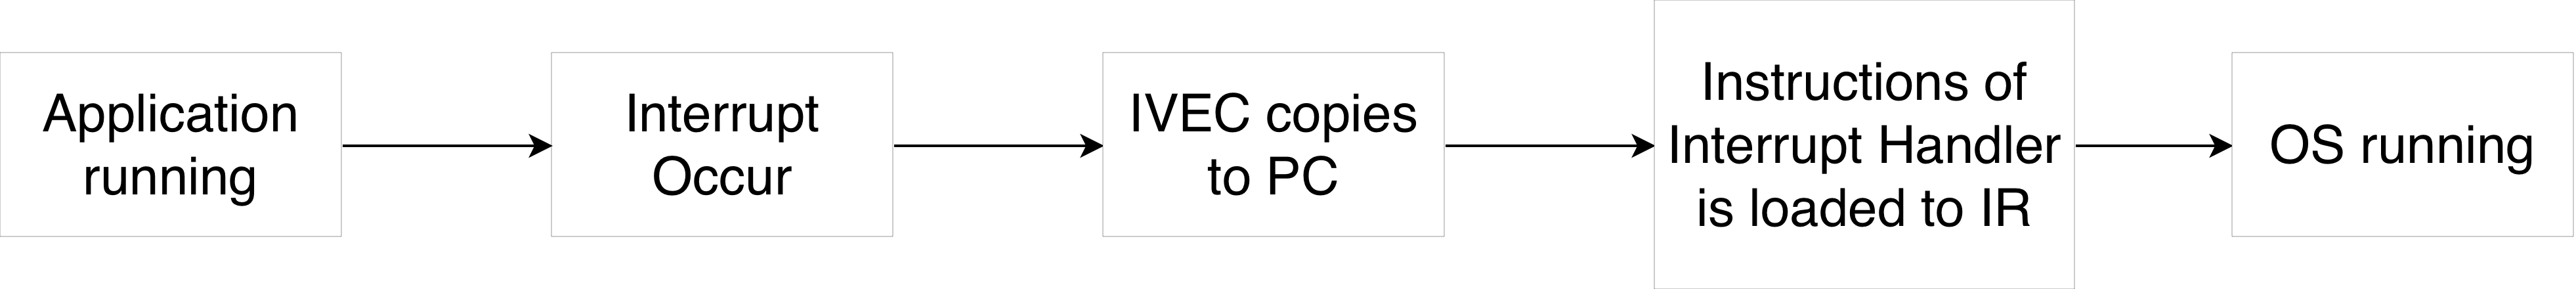
\includegraphics[width=\textwidth]{images/img-04.png}
	\caption{Control transfer from application to OS on an interrupt}
\end{figure}

\subsection{Why Interrupts Matter}
\begin{itemize}
	\item Without interrupts, an application could run forever and hog the CPU.
	\item Keyboard and mouse interrupts happen only when the user acts, so they cannot be relied on. The \textbf{timer} therefore raises an interrupt at regular intervals, guaranteeing that the OS regains control periodically.
\end{itemize}

\begin{extra}[Real hardware]
	A single \reg{IVEC} register is a simplification. On x86 there are many interrupt sources, each with its own handler, so the CPU uses an \emph{interrupt vector table} (the IDT in protected mode), which holds one handler address per interrupt number. The CPU also saves the old \reg{PC} and flags and switches to kernel mode before running the handler.
\end{extra}

\section{x86 Privilege Rings}

\begin{figure}[H]
	\centering
	\begin{minipage}{0.3\textwidth}
		\centering
		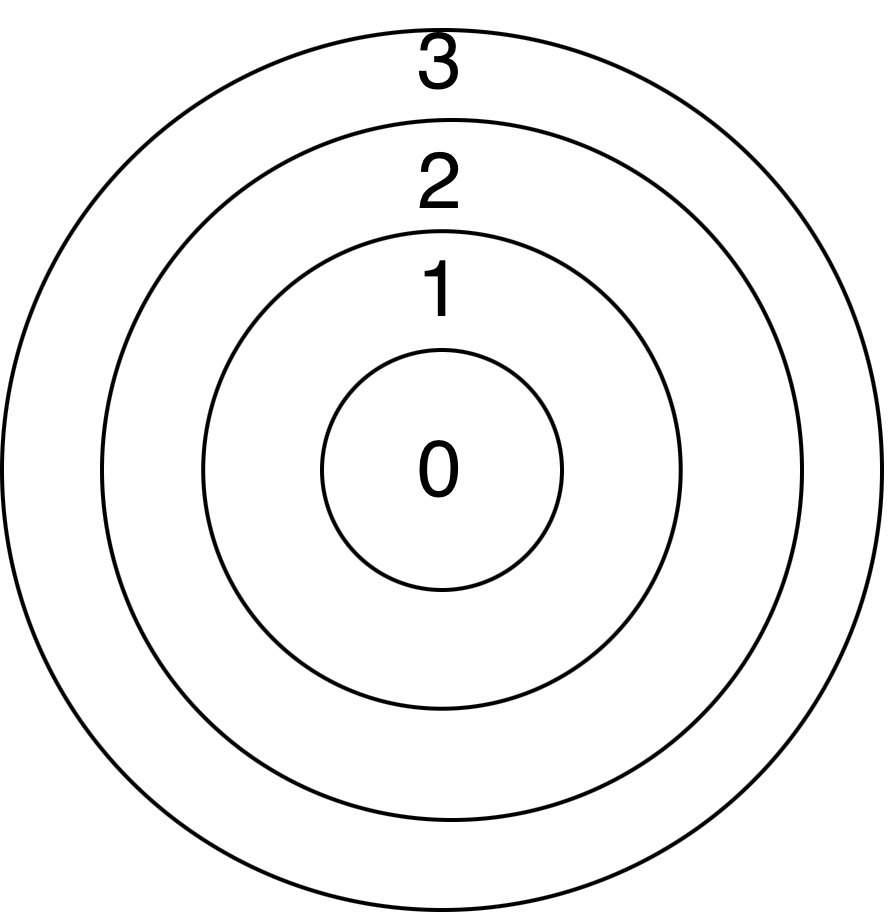
\includegraphics[width=\textwidth]{images/img-05.png}
		\captionof{figure}{x86 protection rings}
	\end{minipage}
	\hfill
	\begin{minipage}{0.6\textwidth}
		\begin{itemize}
			\item The rings are privilege levels: \textbf{0 is the most privileged, 3 the least}.
			\item The CPU uses them to restrict which memory can be accessed and which instructions can be executed, so that buggy or malicious software cannot crash the system.
			\item \textbf{Ring 0 -- Kernel mode:} the OS kernel runs here with unrestricted access to memory and hardware.
			\item \textbf{Rings 1 \& 2:} intended for device drivers and OS services needing intermediate privilege.
			\item \textbf{Ring 3 -- User mode:} applications and user-space processes run here with restricted hardware access and isolated virtual memory.
		\end{itemize}
	\end{minipage}
\end{figure}

\begin{extra}[In practice]
	Mainstream operating systems (Windows, Linux) use only \textbf{ring 0 and ring 3}. Rings 1 and 2 exist in the architecture but are essentially unused.
\end{extra}

\section{Number Representation (Endianness)}

\begin{itemize}
	\item A number that spans multiple bytes has a \textbf{Most Significant Byte (MSB)} and a \textbf{Least Significant Byte (LSB)}.
	\item \emph{Endianness} defines the order in which these bytes are stored in memory.
	\item \textbf{Big endian:} the MSB is stored at the \emph{lowest} address.
	\item \textbf{Little endian:} the LSB is stored at the \emph{lowest} address.
	\item x86 uses \textbf{little endian}.
\end{itemize}

\subsection{Example}
Consider the 4-byte number \texttt{0x12345678}, with MSB $=$ \texttt{12} and LSB $=$ \texttt{78}.

\begin{table}[H]
	\centering
	\begin{tabular}{lcccc}
		\toprule
		\textbf{Address} & \texttt{+0} & \texttt{+1} & \texttt{+2} & \texttt{+3} \\
		\midrule
		Big endian & \texttt{12} & \texttt{34} & \texttt{56} & \texttt{78} \\
		Little endian & \texttt{78} & \texttt{56} & \texttt{34} & \texttt{12} \\
		\bottomrule
	\end{tabular}
\end{table}

\begin{extra}[Why it matters later]
	Endianness affects multi-byte fields on disk too. For example, the MBR signature (Section~\ref{sec:mbr}) is the byte sequence \texttt{55 AA}, which reads as the 16-bit value \texttt{0xAA55} on a little-endian machine.
\end{extra}

\section{Function Calls and the Stack}

\subsection{Saving Registers}
\begin{itemize}
	\item When a function is going to use a register that already holds a value the caller needs, the compiler emits instructions that \texttt{push} the register onto the stack at the start of the function and \texttt{pop} it back at the end.
	\item This preserves the caller's values.
	\item The exact rules (whether caller or callee saves which registers) are defined by the \textbf{calling convention}.
\end{itemize}

\subsection{Example: One-Register Machine}
\begin{minted}{c}
#include <stdio.h>

void func() {
	int x = 0;
	x++;
	printf("%d\n", x);
}

int main() {
	int b = 10;
	func();
	printf("%d\n", b);
	return 0;
}
\end{minted}
The output is \texttt{1} followed by \texttt{10}.

Assume the machine has only one register, \reg{R}, for holding variable values.

\begin{enumerate}
	\item \texttt{main} runs first and stores \texttt{b = 10} in \reg{R}.
	\item The call instruction pushes the \textbf{return address} onto the stack, then sets \reg{PC} to the address of the first instruction of \texttt{func}.
	\item At the start of \texttt{func}, before \reg{R} is reused for \texttt{x}, the old value of \reg{R} (10) is pushed onto the stack.
	\item \texttt{func} sets \reg{R} to 0, increments it to 1 and prints it.
	\item Before returning, \texttt{func} pops the saved value back into \reg{R}, so \reg{R} holds 10 again.
	\item The return instruction pops the return address into \reg{PC}, and \texttt{main} resumes where it left off and prints 10.
\end{enumerate}

\begin{table}[H]
	\centering
	\begin{tabular}{cl}
		\toprule
		\textbf{Stack (top first)} & \textbf{State} \\
		\midrule
		\texttt{saved R = 10} & after the push inside \texttt{func} \\
		\texttt{return address} & pushed by the call \\
		\bottomrule
	\end{tabular}
\end{table}
Values are popped in the reverse order they were pushed (LIFO): the saved register first, then the return address.

\section{Booting}

\subsection{Power-On}
\begin{itemize}
	\item RAM contents are undefined at power-on. Most registers also hold arbitrary values, but the hardware resets a few (including \reg{PC}) to defined values.
	\item \reg{PC} is set to a fixed \textbf{reset vector} in ROM. ROM is non-volatile, so unlike RAM its contents survive power loss.
	\item On classic x86 the reset vector is 16 bytes below the top of the address space. These 16 bytes hold a jump to the entry code of the \textbf{BIOS} firmware. This indirection allows different machines to have different ROM sizes and layouts.
	\item The BIOS runs in real mode with unrestricted hardware access (the privilege rings do not apply yet).
\end{itemize}

\subsection{Boot Sequence}
\begin{enumerate}
	\item \textbf{POST} (Power-On Self Test): the BIOS checks that the hardware is present and working.
	\item The BIOS reads the \textbf{first sector} of the boot disk into RAM. This is the MBR (Section~\ref{sec:mbr}).
	\item The BIOS jumps to the start of that code in RAM (the \emph{boot call}).
	\item The MBR code loads a \textbf{bootloader} (directly, or via a second stage or the active partition's boot sector).
	\item The bootloader loads the \textbf{OS kernel} into memory and jumps to it.
	\item The kernel sets up its own interrupt handlers (writes \reg{IVEC} / the interrupt vector table) and finishes initialization.
\end{enumerate}

\begin{extra}[UEFI]
	Modern machines use UEFI firmware instead of the legacy BIOS and typically a GPT partition scheme instead of the MBR. The overall idea (firmware $\rightarrow$ bootloader $\rightarrow$ kernel) is the same.
\end{extra}

\subsection{Master Boot Record (MBR)}
\label{sec:mbr}
Consider a disk with 512-byte sectors. The MBR is the first sector.

\begin{table}[H]
	\centering
	\begin{tabular}{lll}
		\toprule
		\textbf{Offset} & \textbf{Size} & \textbf{Content} \\
		\midrule
		0 & 446 bytes & Boot code \\
		446 & 64 bytes & Partition table (4 entries $\times$ 16 bytes) \\
		510 & 2 bytes & Boot signature: \texttt{55} at 510, \texttt{AA} at 511 (written 0x55AA) \\
		\bottomrule
	\end{tabular}
\end{table}

\begin{itemize}
	\item The signature marks the sector as bootable. Read as a little-endian 16-bit word it is \texttt{0xAA55}.
	\item The table holds up to \textbf{4 primary partitions}.
\end{itemize}

\paragraph{Partition entry (16 bytes).}
\begin{table}[H]
	\centering
	\begin{tabular}{lll}
		\toprule
		\textbf{Field} & \textbf{Size} & \textbf{Meaning} \\
		\midrule
		Status & 1 B & \texttt{0x80} = active (bootable), \texttt{0x00} = inactive \\
		Start CHS & 3 B & Start address in cylinder/head/sector form \\
		Type & 1 B & Partition type code \\
		End CHS & 3 B & End address in CHS form \\
		Start LBA & 4 B & First sector, as a logical block address \\
		Sector count & 4 B & Size of the partition in sectors \\
		\bottomrule
	\end{tabular}
\end{table}
\begin{itemize}
	\item There is no stored partition number; it is implied by the entry's position in the table.
	\item The type is a \emph{code}, not a filesystem name. For example \texttt{0x07} is NTFS/exFAT and \texttt{0x83} is Linux (used for ext4). A code can map to several filesystems.
\end{itemize}

\begin{extra}[Magic numbers]
	A \textbf{magic number} is a fixed byte pattern at the start of a file that identifies its format. On Linux, the kernel uses it to decide how to run an executable, and the \texttt{file} command uses it (plus other heuristics) to identify files. The file extension does not matter.
	\begin{itemize}
		\item ELF executables: \texttt{0x7F} followed by \texttt{ELF}
		\item Java class files: \texttt{0xCAFEBABE}
		\item Scripts: \texttt{\#!} (the magic) followed by an interpreter path, e.g.\ \texttt{\#!/bin/bash}. The path can be any interpreter.
	\end{itemize}
\end{extra}


\appendix
\section{Glossary}

\begin{table}[H]
	\centering
	\begin{tabular}{lp{0.7\textwidth}}
		\toprule
		\textbf{Term} & \textbf{Meaning} \\
		\midrule
		\reg{PC} & Program counter: address of the next instruction \\
		\reg{IR} & Instruction register: the instruction being executed \\
		\reg{IVEC} & Interrupt vector register: address of the interrupt handler \\
		BIOS & Firmware in ROM that starts the boot process \\
		POST & Power-On Self Test, run by the BIOS \\
		MBR & Master Boot Record: first sector of a disk \\
		MSB / LSB & Most / least significant byte \\
		LIFO & Last in, first out (stack order) \\
		\bottomrule
	\end{tabular}
\end{table}


\end{document}
